\chapter{Literature Review}
\label{chap:lr}

This chapter gives information about the concepts and techniques that we will use.
In addition, we provide a summary of the most common tools for visualizing Rust source code.
Section \ref{sec:vis} describes the notion of visualization, its examples, and its types.
Section \ref{sec:html} gives a brief description of the HTML language that we will use to build the final report.
In section \ref{sec:rust} we talk about Rust, and why we decided to choose this language.
Section \ref{sec:anal} discusses how to perform static analysis of Rust code.
Section \ref{sec:sol} presents the most popular existing solutions for visualization, describes and evaluates them.
We make a conclusion about visualization and current solutions, describing their advantages and disadvantages in section \ref{sec:conc}.


% Software development is a rather complicated and not straightforward task. 
% In big projects, there are thousands of lines of code and hundreds of files in which a programmer should be able to understand what is happening to develop or maintain the project. 
% To fulfill this need, program visualization was introduced.

\section{Source code visualization}
\label{sec:vis}
In big projects, there are thousands of lines of code and hundreds of files in which a programmer should be able to understand what is happening to develop or maintain the project. 
To fulfill this need, program visualization was introduced.

Program visualization is a mapping from programs to graphical representations \cite{247643}. Architecture diagrams, dependency graphs, and, code visualization help to see the overall picture presented in the program. 
For example, \cite{cvsscan} introduces visualization of code evolution. It is an integrated environment to track code changes, the contributors' roles, and the history of a project using line-oriented displays.
ViLLE \cite{ville} is another example of program visualization. It has several features, for example, code editing, tracing execution, code line explanation, and language-independency. Also, ViLLE team conducted research and concluded that code visualization improves students' learning regardless of their programming skills.

There are several types of program visualization. The most popular one is text visualization which is offered by many IDE.
It consists of all possible options for modifying the source code, for example, adding hints in the text, coloring keywords or other tokens, accentuating logical blocks, icons, color highlights, and code navigation \cite{2018visual}. 
Figure \ref{fig:hl_example_1} shows an example of visualizing a source code. Here end user can see, for example, highlighted syntax, and additional information about the types of variables and functions documentation.

Source code visualization is quite popular nowadays since it provides detailed information about the project. In addition, it is a useful tool for newcomers to overcome the barrier of a huge amount of information available at the start \cite{5336433}. 

To sum up, program visualization is a popular and useful tool for developing and maintaining a projects. 
There are several types and examples of visualization. Text visualization is widely used by developers today because it offers an intuitive environment for navigating and explaining code.

\begin{figure}[hbt]
\centering
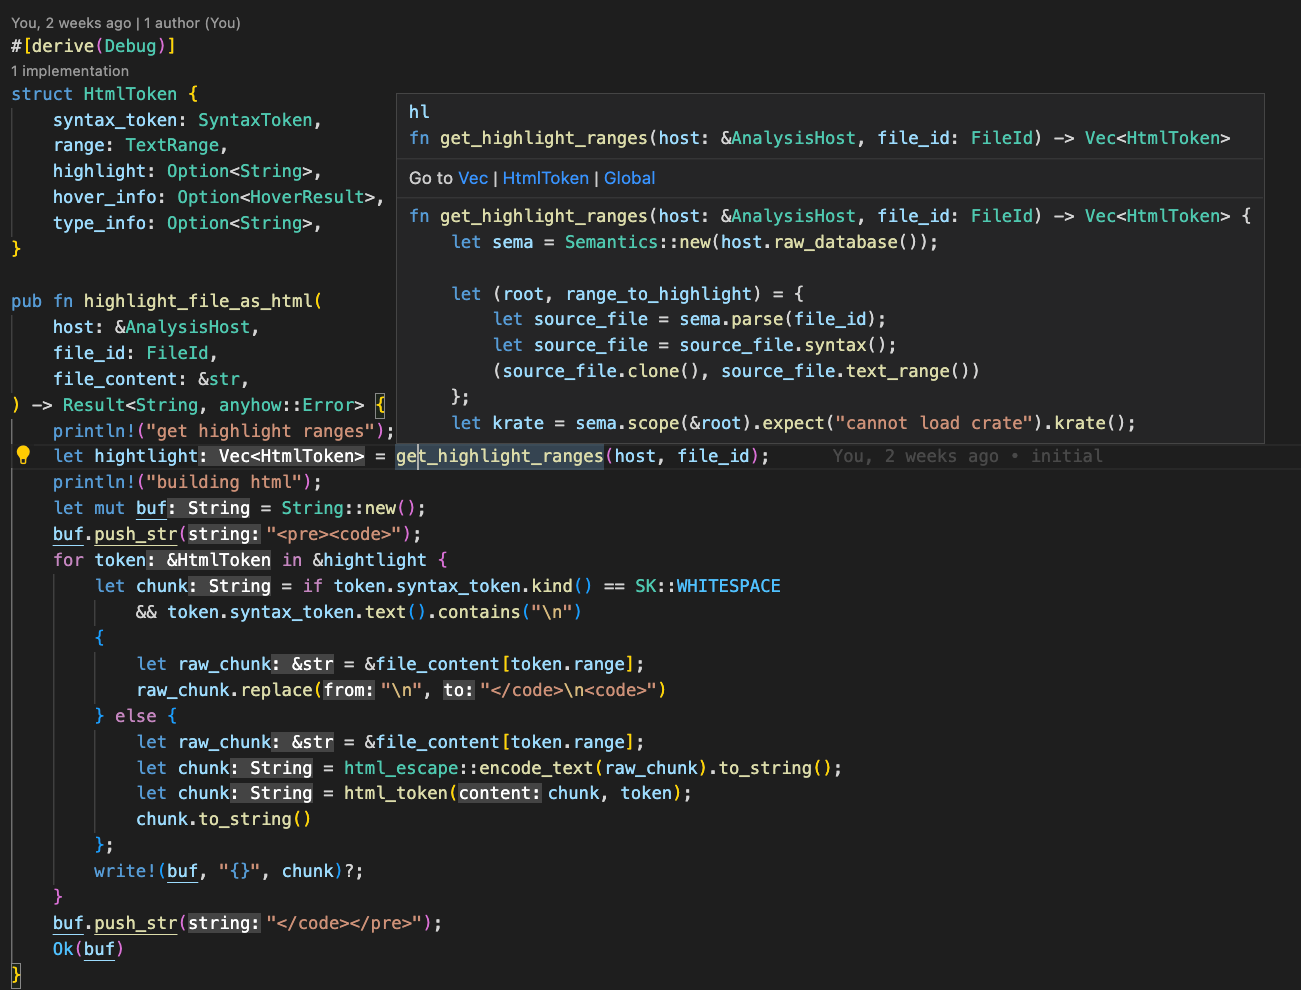
\includegraphics[width=15cm]{figs/hl_example_2.png}
\caption{Source code visualization example}
\label{fig:hl_example_1}
\end{figure}



\section{Visualization via HTML}
\label{sec:html}

HTML is the markup language for creating Web pages. It can be used for text visualization. It has a lot of built-in features that will help us to implement all the visualization features that we want. The main advantage of HTML over other visualization methods is that it is popular and widely used. Every modern browser can show an HTML page without additional dependencies and internet access.
Visualization via HTML is quite popular nowadays. 
GitHub \cite{github} is web storage of source code, that supports HTML highlighting for over 1000 languages.
Another example is \textit{Online Python Tutor}. It is a web-based program visualization tool for Python \cite{python}. Using that tool users can write programs in the browser with a visualization of each execution step.

% \section{Program static analysis}
% \label{sec:2anal}


% TODO: too small
% how it's related to visualization


\section{The Rust language}
\label{sec:rust}
Rust is a new programming language for developing reliable and efficient systems \cite{rust-official}.
Currently, Rust is gaining popularity, and some companies prefer it rather than C++ \cite{top-lang}. 

Rust provides a wide range of high-level features, such as static typing, thread, and memory safe together with low-level features such as full memory control.
Rust has 48 keywords (31 currently used keywords and 17 reserved for future use). For example, in the C++ language that is most similar to Rust in terms of application area, there are 95 keywords which are almost twice as many. 
There are no header files in Rust and a big project can be divided into encapsulated crates and modules that provide convenient and readable architecture. 
Rust developers were able to make a memory-safe system without a garbage collector using compiler-checked abstractions. A strong ownership system ensures programmers that, for example, there will not be a memory leak, uninitialized memory access or data-race problem \cite{reed2015patina}.
Another advantage of choosing Rust as the language for this study is that although it is a complex syntactic language, it provides an open API for static code analysis, so the development of a code visualizer will not go into the task of developing its compiler.
But at the same time, Rust also has drawbacks: it has a rather complex syntax for beginners and it lacks a lot of user libraries, due to its novelty.

To sum up, we decided to choose Rust language because it is modern, relatively popular, and powerful. Using that language big and complicated projects can be built, so code visualization would be helpful in this situation.

\section{Rust source code analysis}
\label{sec:anal}
Static analysis is strongly connected to source code visualization. In order to visualize the program code, we should represent the code in a more informative data structure. For this purpose, source code parsing, the first step of every static analysis approach, is used. This is a process of representing a set of characters into a more abstract and useful data structure, for example, an Abstract Syntax Tree (AST). 

Static program analysis is a way to analyze a program without running it. It takes source code and produces a report, for example, a bug report in software \cite{anal}. MirChecker \cite{mirchecker} is an example of applying static analysis of MIR (mid-level intermediate representation provided by Rust compiler) to automatically find bugs in Rust programs. 

The programming language syntax is a set of language rules. It defines how to write valid programs and what is the structure of these programs. As was mentioned before, Rust has a fairly rich syntax that allows users to use complex constructs such as generic, macros, error propagation, lambda functions, a lifetime of variables, and many others. 
Because of this, for beginners, Rust may seem complicated and even verbose. However, in this case, highlighting tokens could be helpful for newcomers.

\textit{Syn} is a Rust crate that is used to parse a stream of tokens into a Rust syntax tree and its main purpose is to write procedural macros in Rust \cite{crates-syn}. 
\textit{Rust-analyzer} is a set of crates for semantic analysis of Rust code. It uses MIR analysis internally and provides API to analyze source code and obtain meta information about tokens, such as definition place, references, and inferred type information \cite{crates-rust-analyzer}. Later, in the methodology section, we will discuss how those crates will help us build the parsing module of our application.

% Nevertheless, complicated syntax is problem for parsing and static analyzing and Rust solves this problem by introducing high-level intermediate mid-level intermediate representation (MIR) of source code. This presentation can be obtained from the compiler and represented as modified source code with expanded macros, explicit types and simplified constructions. 
Summing up, static analysis is closely related to text visualization. Rust syntax is quite complicated, however, Rust offers clear API to perform source code analysis.

\section{Existing solutions}
\label{sec:sol}

In this section, we will discuss existing solutions for Rust code visualization, and understand what their disadvantages are.

\begin{enumerate}[label=\arabic*)]
    \item \textbf{Visual Studio Code extension} - Rust has its own extension for VSCode IDE. The extension is built on top of the \textit{rust-analyzer} \cite{crates-rust-analyzer} library. It provides some of the required functionality via the Language Server Protocol, however, it is geared toward writing code, and, therefore, requires installation of VSCode, its dependencies, and the extension itself. In addition, there is no portable output of the project, so this solution is powerful, but not appropriate for our case.

    \item \textbf{Rustdoc} - is a tool to generate HTML documentation for Rust source code \cite{rustdoc}, for example, additional comments for modules, function signatures, and trait implementations. It also provides a feature to browse source code. However, it lacks many useful features, for example, identifier information, jumps to references, and type of variables. Also, it shows \textit{.rs} files only, which is logical for documentation purposes, but inconvenient for a full understanding of the project.

    \item \textbf{github.com} - Internet hosting site for version control system \cite{github}. Used to store source code of projects. It provides basic highlighting and static code analysis such as showing definitions and references. However it requires loading every source code page over the internet, it doesn't have a project tree and it has the least number of visualization features of all the solutions presented since visualization is a secondary feature of GitHub.
\end{enumerate}

% github.com - only highlitgh

% vscode + rust-analyzer -- very powerful, but havy, doesn't produce static file

% rustdoc - similar to what we want, but lack of some usefull features
% novelty
% to the best of our knowledge, there is no existing solution 
% we offer 

\section{Conclusion}
\label{sec:conc}

In conclusion, among the many types of visualization, we decided to choose text visualization as the most popular and widely used. 
There are solutions in the field of Rust code text visualization, however, they all lack usability or portability, or they require the installation of many dependencies since they indented to write and change the source code.
Our solution is to use a portable and cross-platform visualization format such as HTML and use all the known useful features to explore the program text conveniently.

\newpage

